\documentclass[a4paper,11pt]{article}
\usepackage[left=2cm,text={17cm, 24cm},top=3cm]{geometry} 
\usepackage{times}
\usepackage[czech]{babel}
\usepackage[utf8]{inputenc}
\usepackage{multirow}
\usepackage{graphics}
\usepackage{picture}
\usepackage[pdftex]{lscape}
\pagestyle{plain}
\bibliographystyle{czechiso}
\pagenumbering{arabic}

\begin{document}
	\begin{titlepage}
		\begin{center} \Huge \textsc{Vysoké učení technické v Brně \\ \huge Fakulta informačních technologií\\} 
			\vspace{\stretch{0.382}} \LARGE Formální jazyky a překladače \\ \Huge Implementace překladače imperativního jazyka IFJ19 \vspace{\stretch{0.618}} 
			
			\end{center}	

		{\LARGE \today}
	\end{titlepage}
	\newpage
	\tableofcontents
    \newpage


\section{Úvod}
Cílem projektu je tvorba programu v jazyce C, který  je podmnožinou jazyka Python 3. Načítá zdrojový kód zapsaný ve zdrojovém jazyce IFJ19 a překládá jej do cílového jazyka IFJcode19 (mezikód).

\section{Návrh a~implementace}
Projekt se skládá ze čtyř hlavních částí, které spolu navzájem spolupracují.

\subsection{Lexikální analýza}
Lexikální analýza provádí skenování vstupního kódu Python 3, který uživatel vkládá při spouštění programu. Jedná se o první část programu provádějícího překlad abstraktního programovacího jazyku Python 3 do IFJcode19 a zastává práci deterministického automatu, který parsuje jednotlivé lexémy, provádí jejich kontrolu a vyhodnocuje jejich význam. Výstupem lexikální analýzy je typ a hodnota každého lexému.
\\
Implementace:\\
Lexikální analyzátor je implementován podle zadání projektu v jazyce C a nachází se v souborech \textit{lexical_analysis.h} a \textit{lexical_analysis.c}. 
\\
LEXICAL_ANALYSIS.H
V hlavičkovém souboru nalezneme definici struktury \texttt{Symbol}, která je výstupem analyzátoru a obsahuje v sobě hodnoty \texttt{Type} a \texttt{Data}. 
Type udává výčet typů, kterých parsovaný lexém může nabývat. Příkladem může být: \textit{integer, string, function, double,} atd..
Data jsou typu \texttt{union}, jež obsahuje jeden z datových typů integer, double nebo char*. Tato hodnota je závislá na typu lexému. Pokud tedy načteme například číslo 5, tak jeho typem bude integer a hodnota bude číslo 5 uložena v unionu jako integer. Pro případ řetězce, by to pak byl typ string a hodnota v unionu uložena jako char*. Díky tomuto zápisu můžeme vracet různé hodnoty podle nahraného datového typu. \\

Dále zde nalezneme výčet všech možných stavů, do kterých se lexikální analyzátor může dostat. Tento seznam je shodný s konečným automatem. \\

\begin{figure}[h]
\begin{center}
{\scalebox{0.5}
{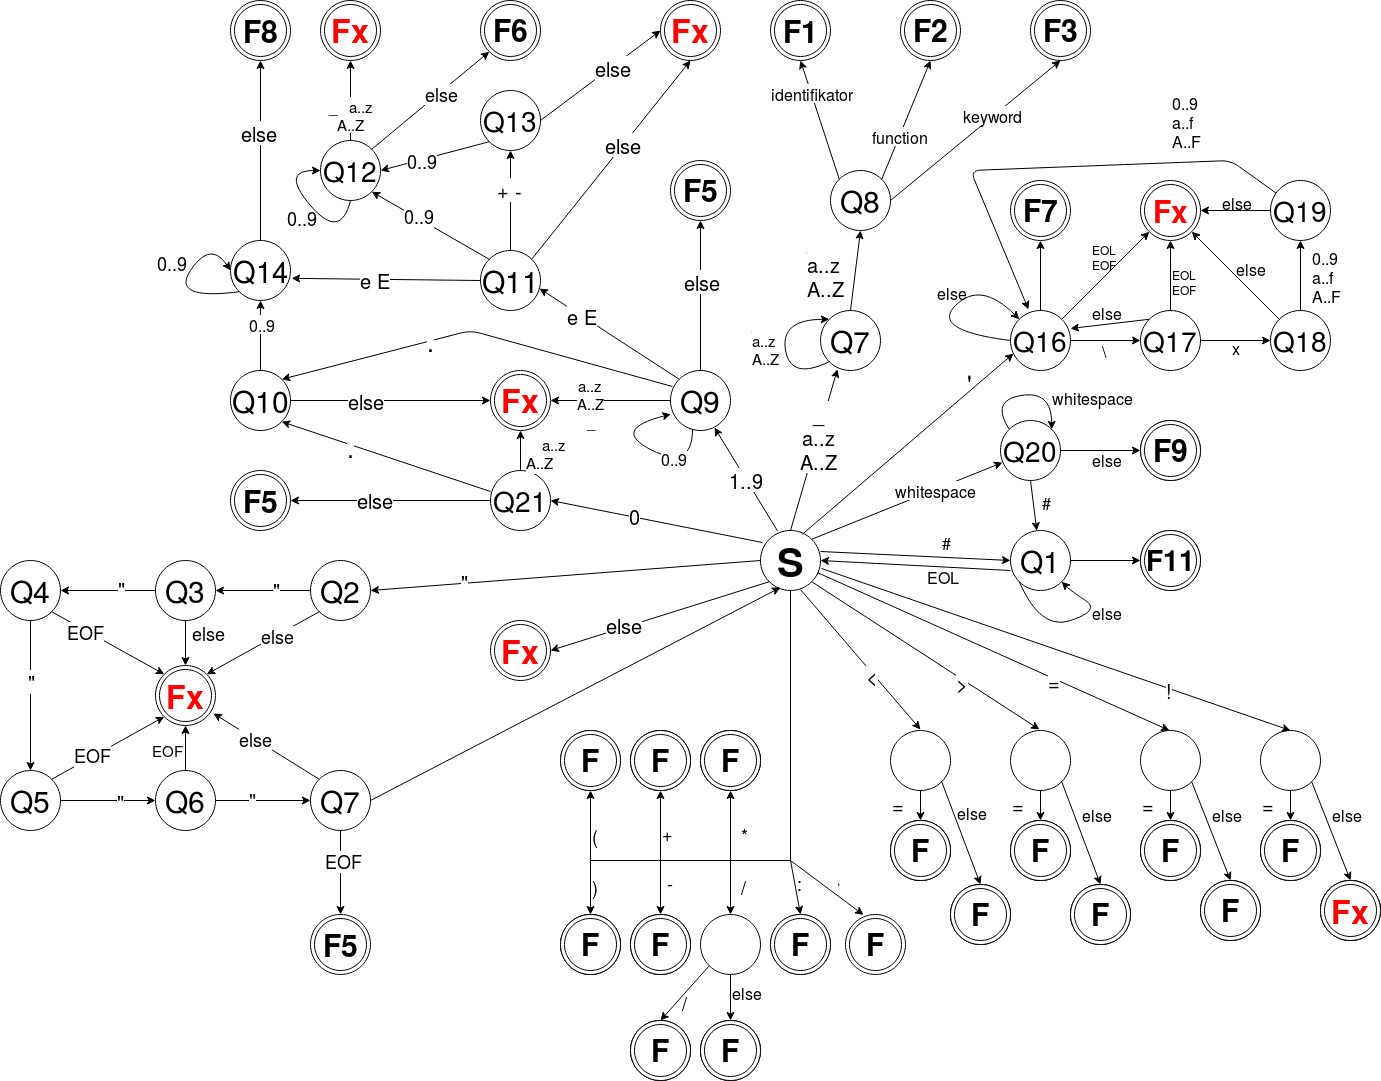
\includegraphics{ka.png}}}
\label{obr}
\caption{Konečný automat}
\end{center}
\end{figure}
\\

LEXICAL_ANALYSIS.C
Obsahuje implementaci funkcí pro práci s lexémy. Hlavní funkce, která parsuje lexémy se nazývá \texttt{getNextSymbol} a její předpis je následující: \\
\textt{struct Symbol getNextSymbol(FILE*);}
Můžeme si tedy všimnout, že parametrem je datový typ \texttt{FILE*}, neboli ukazatel na soubor, ze kterého máme číst vstupní kód (nebo hodnota stdin).
Parsování probíhá v neustále se opakujícím while cyklu, který se pomocí přepínače posouvá ze stavu do stavu podle nahrávaných hodnot. Čtení se provádí po jednotlivých znacích a je neustále vyhodnocována správnost nahrávaného lexému. Ten je obvykle ukončen mezerou, znakem konce řádku, nebo znakem konce souboru. V takovém případě pak vrátíme zjištěná data pomocí struktury \texttt{Symbol}.



\section{Závěr}



\newpage
\bibliography{ref}
\end{document}
